\documentclass[slidestop,compress,mathserif]{beamer}

\usepackage{kotex}
\usepackage{graphicx}
\usepackage{authblk}
\usepackage{mdframed}
\usepackage{amsmath}
\usepackage{amsfonts}
\usepackage{amsthm}
\usepackage{mathrsfs}
\usepackage{setspace}
\usepackage{proof}
\usepackage{hyperref}

\author{ 임기정 }
\title{$\lambda$Prolog로 나만의 타입체커 만들기}

\hypersetup{ colorlinks=true, linkcolor=blue, filecolor=magenta, urlcolor=cyan, }

\newenvironment{nemochang}
{
    \begin{center}
    \begin{tabular}{|p{0.95\textwidth}|}
    \hline
    \vspace{0.1em}
}
{
    \hline
    \end{tabular}
    \end{center}
}

\begin{document}
    \begin{frame}
        \titlepage
    \end{frame}

    \begin{frame}
        \frametitle{서론}
        \begin{itemize}
            \item 타입체커를 쉽게 만들고자 하시는 분들을 위해 발표합니다!
            \pause
            \item System-F:
            \begin{enumerate}
                \item 단순 타입 람다-계산법에 타입에 대한 보편 양화사를 추가한 시스템입니다.
                \item 하스켈과 ML 같은 함수형 언어의 이론적 기반입니다.
            \end{enumerate}
            \pause
            \item 논리형 프로그래밍:
            \begin{enumerate}
                \item \textit{규칙}이라 불리는 논리식들을 작성하는 프로그래밍 패러다임입니다.
                \item 그리하여 인터프리터가 그 규칙들로부터 질의받은 논리식을 증명할 수 있는지를 응답합니다.
            \end{enumerate}
            \pause
            \item $\lambda$Prolog:
            \begin{enumerate}
                \item 람다-식을 매칭할 수 있다는 게 가장 두드러지는 특징인 논리형 프로그래밍 언어입니다.
                \item 가장 유명한 구현체로는 Teyjus가 있는데, 본 발표에서는 \href{https://github.com/teyjus/teyjus/releases}{[링크]}에서 다운받을 수 있는 Teyjus V2를 사용할 것입니다.
            \end{enumerate}
        \end{itemize}
    \end{frame}
    
    \begin{frame}
        \frametitle{$\lambda$Prolog의 구문론}
        \begin{itemize}
            \item $\lambda$Prolog의 타입체계는 STLC에 랭크 1의 타입을 허용한 것이며, ad-hoc 다형성을 지원합니다.
            \item 변수 $x$: 하스켈과 반대로, 대문자로 시작하는 식별자입니다.
            \item 상수 $c$: 하스켈과 반대로, 소문자로 시작하는 식별자입니다.
            \item 항 $t$:
            \begin{enumerate}
                \item $t$ \texttt{::=} $x$: 변수은 항입니다.
                \item $t$ \texttt{::=} $c$: 상수는 항입니다.
                \item $t$ \texttt{::=} ($t$ $t$): 적용은 항입니다.
                \item $t$ \texttt{::=} ($x$\texttt{\string\ }$t$): $\lambda$-추상은 항입니다.
            \end{enumerate}
            \item 원자 논리식 $A$: 타입이 $o$인 항입니다.
            \begin{enumerate}
                \item 술어: 원자 논리식 $A$의 HNF는 $\left( \left( \left( p \, t_1 \right) \, \cdots \, \right) \, t_n \right)$ 꼴인데, 여기서 $p$를 $A$의 술어라고 합니다. 단, $n \geq 0$.
                \item 엄격한 원자 논리식 $A_r$: 술어가 상수인 원자 논리식입니다.
            \end{enumerate}
        \end{itemize}
    \end{frame}

    \begin{frame}
        \frametitle{$\lambda$Prolog의 구문론}
        \begin{itemize}
            \item 질의 $G$:
            \begin{enumerate}
                \item $G$ \texttt{::=} $A$은 $A$를 뜻합니다.
                \item $G$ \texttt{::=} \texttt{true}은 $\top$을 뜻합니다.
                \item $G$ \texttt{::=} $G_1$\texttt{,} $G_2$은 $G_1 \land G_2$을 뜻합니다.
                \item $G$ \texttt{::=} $G_1$\texttt{;} $G_2$은 $G_1 \lor G_2$을 뜻합니다.
                \item $G$ \texttt{::=} $D_1$ \texttt{=>} $G_2$은 $D_1 \supset G_2$을 뜻합니다.
                \item $G$ \texttt{::=} \texttt{pi} $x_1$\texttt{\string\ }$G_2$은 $\forall x_1 . G_2$을 뜻합니다.
                \item $G$ \texttt{::=} \texttt{sigma} $x_1$\texttt{\string\ }$G_2$은 $\exists x_1 . G_2$을 뜻합니다.
            \end{enumerate}
            \item 규칙 $D$:
            \begin{enumerate}
                \item $D$ \texttt{::=} \texttt{pi} $x_1$\texttt{\string\ }$D_2$은 $\forall x_1 . D_2$을 뜻합니다.
                \item $D$ \texttt{::=} $A_r$은 $A_r$을 뜻합니다.
                \item $D$ \texttt{::=} $A_r$ \texttt{:-} $G$은 $G \supset A_r$을 뜻합니다.
            \end{enumerate}
            \item 이러한 질의와 규칙들의 언어를 \textit{higher-order hereditary Harrop}(또는 줄여서 \textit{hohh})라고 합니다.
        \end{itemize}
    \end{frame}

    \begin{frame}
        \frametitle{시그니처}
        \begin{itemize}
            \item 이제 타입체커의 시그니처 파일을 다음과 같이 작성해봅시다.
            \begin{figure}[h]
                \begin{center}
                    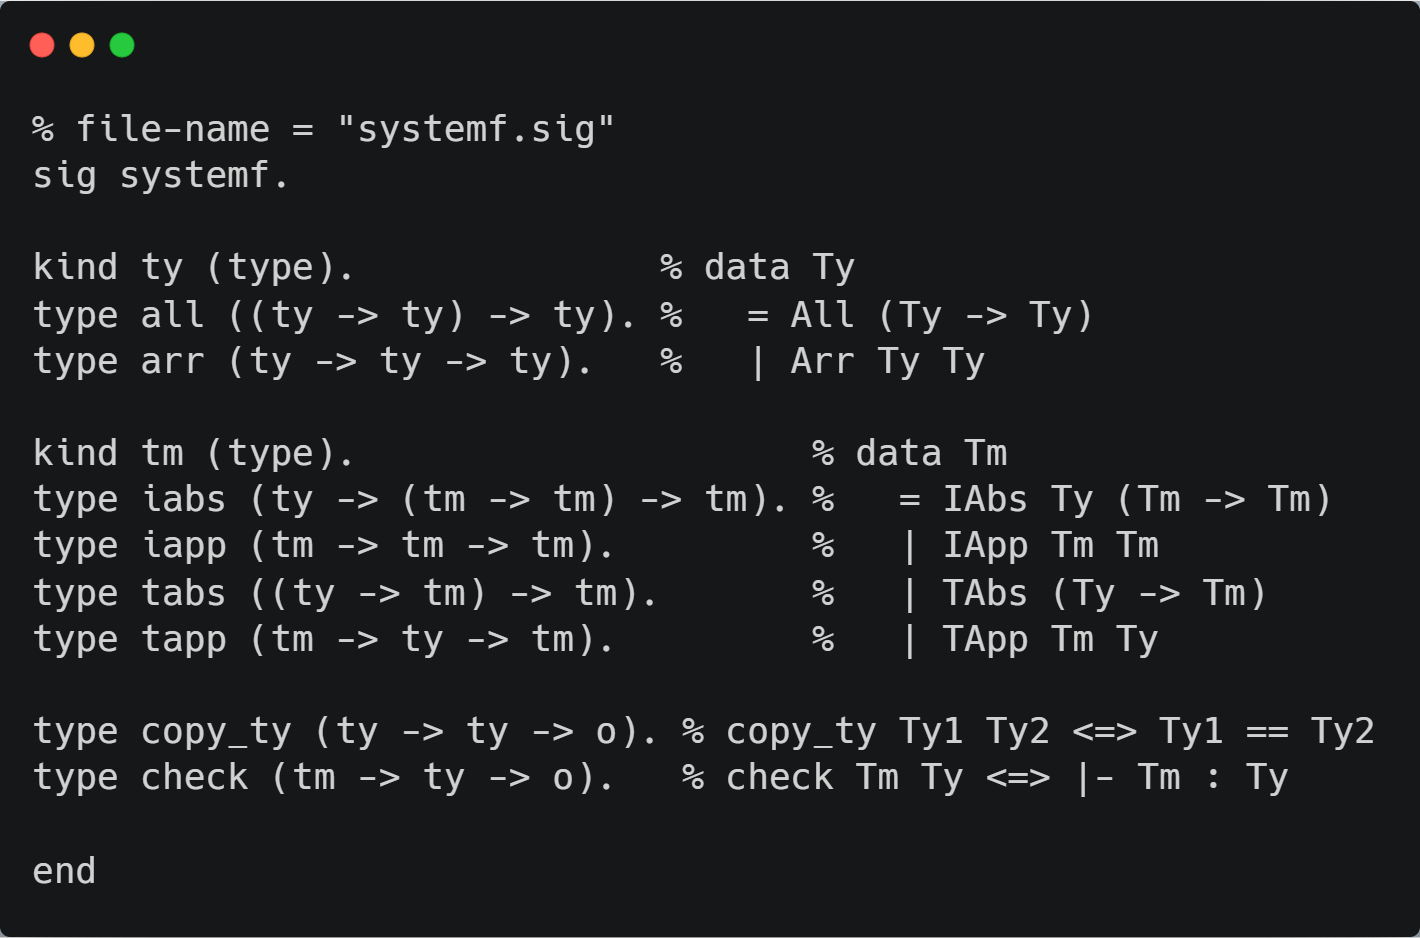
\includegraphics[width=0.7\linewidth]{sig.png}
                \end{center}
            \end{figure}
            \item 저기서 \texttt{\%}와 그 뒤에 오는 문자들은 주석 처리되기 때문에 적지 않으셔도 됩니다.
        \end{itemize}
    \end{frame}

    \begin{frame}
        \frametitle{시그니처}
        \begin{itemize}
            \item 이제부터 이 코드의 의미를 알아봅시다.
            \item 우리는 닫힌 타입과 닫힌 항만의 System-F의 타입체커를 짤 것입니다 -- 즉, 우리가 다룰 항과 타입에 자유변수가 없다고 간주합니다.
        \end{itemize}
    \end{frame}

    \begin{frame}
        \frametitle{시그니처}
        \begin{itemize}
            \item 먼저, System-F의 타입을 인코딩한 타입 생성자 \texttt{ty}에 대하여 알아봅시다.
            \item \texttt{ty}의 kind가 \texttt{*}로 선언되어 있고, 그 밑으로는 \texttt{ty}의 자료 생성자가 선언되어 있습니다.
            \item \texttt{all} ($\alpha$\texttt{\string\ }$\sigma$)는 $\left( \forall \alpha . \sigma \right)$를 인코딩한 것이며,
            \item \texttt{arr} $\tau$ $\sigma$는 $\left( \tau \to \sigma \right)$를 인코딩한 것입니다.
        \end{itemize}
    \end{frame}

    \begin{frame}
        \frametitle{시그니처}
        \begin{itemize}
            \item 그 다음, System-F의 항을 인코딩한 타입 생성자 \texttt{tm}에 대하여 알아봅시다.
            \item \texttt{tm}의 kind가 \texttt{*}로 선언되어 있고, 그 밑으로는 \texttt{tm}의 자료 생성자가 선언되어 있습니다.
            \item \texttt{iabs} $\tau$ ($x$\texttt{\string\ }$M$)은 $\left( \lambda x^{\tau} . M \right)$을 인코딩한 것입니다.
            \item \texttt{iapp} $M$ $N$은 $\left( M N \right)$을 인코딩한 것입니다.
            \item \texttt{tabs} ($\alpha$\texttt{\string\ }$M$)은 $\left( \Lambda \alpha . M \right)$을 인코딩한 것입니다.
            \item \texttt{tapp} $M$ $\tau$는 $\left( M \tau \right)$를 인코딩한 것입니다.
        \end{itemize}
    \end{frame}

    \begin{frame}
        \frametitle{시그니처}
        \begin{itemize}
            \item 마지막으로, 다음 두 술어가 선언되어 있는 걸 보실 수 있습니다.:
            \item \texttt{copy\_ty}: 타입 \texttt{ty -> ty -> o}의 술어로서 $\sigma \left[ \alpha := \tau \right]$와 $\tau$로부터 가능한 ($\alpha$\texttt{\string\ }$\sigma$)를 모두 찾기 위해 필요합니다.
            \item \texttt{check}: 타입 \texttt{tm -> ty -> o}의 술어로서 $\vdash M : \sigma$일 때 그리고 그럴 때에만 \texttt{check} $M$ $\sigma$이 성립하도록 구현할 것입니다.
        \end{itemize}
    \end{frame}

    \begin{frame}
        \frametitle{구현}
        \begin{itemize}
            \item 이제 타입체커의 모듈 파일을 다음과 같이 작성해봅시다.
            \begin{figure}[h]
                \begin{center}
                    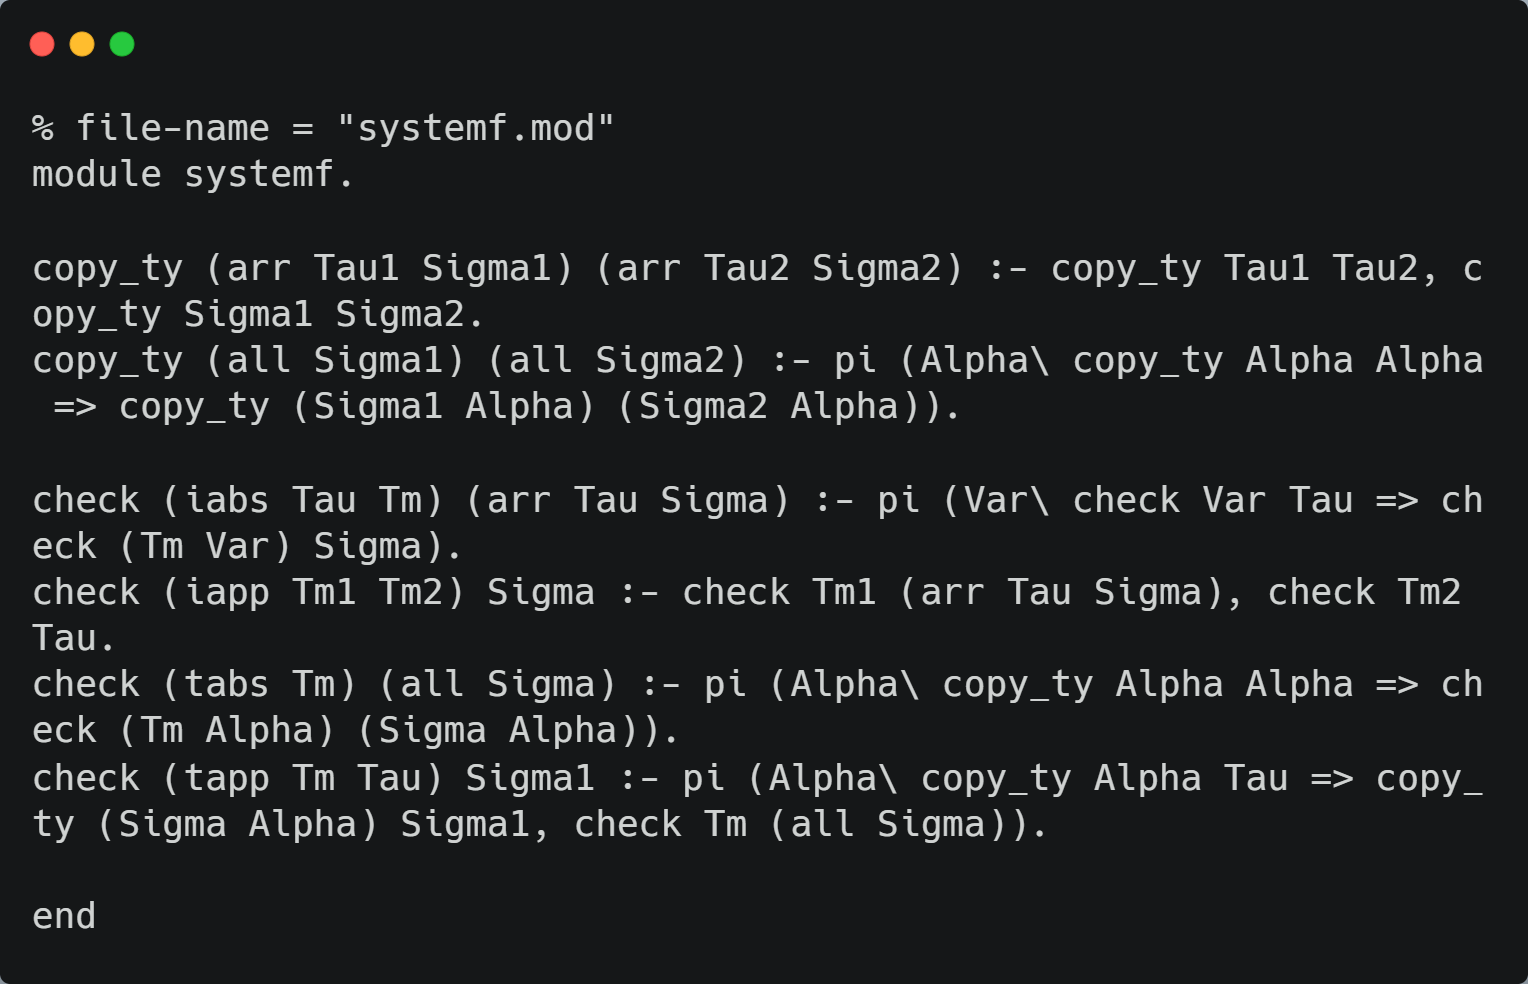
\includegraphics[width=1.0\linewidth]{mod.png}
                \end{center}
            \end{figure}
            \item 이제부터 이 코드의 의미를 알아봅시다.
        \end{itemize}
    \end{frame}

    \begin{frame}
        \frametitle{구현}
        \begin{itemize}[<+->]
            \item 먼저, \texttt{copy\_ty}의 구현부터 봅시다.
            \item 첫 번째 규칙의 의미는 그리 어렵지 않네요:
            \begin{enumerate}
                \item $\tau_2$이 $\tau_1$의 복사본이고
                \item $\sigma_2$이 $\sigma_1$의 복사본이면,
                \item $\tau_2 \to \sigma_2$은 $\tau_1 \to \sigma_1$의 복사본이다.
            \end{enumerate}
            \item 당연한 소리네요.
            \item 두 번째 규칙의 의미를 살펴봅시다:
            \begin{enumerate}
                \item 타입 \texttt{ty}의 새로운 상수 기호 $c$를 도입하고, $c$는 $c$의 복사본이라고 하자.
                \item 이때, $\tau_2 \left[ \alpha := c \right]$가 $\tau_1 \left[ \alpha := c \right]$의 복사본이면,
                \item $\forall \alpha . \tau_2$는 $\forall \alpha . \tau_1$의 복사본이다.
            \end{enumerate}
            \item 이렇게 새로운 상수 기호 $c$를 도입하는 이유는 재귀를 하기 위해 \texttt{ty -> ty}를 \texttt{ty}로 바꿔주기 위함이고,
            \item $c$는 $c$의 복사본이라는 규칙을 추가하는 이유는 재귀의 기저 단계에서 필요하기 때문입니다.
            \item 이제 \texttt{check}의 구현을 살펴보겠습니다.
        \end{itemize}
    \end{frame}

    \begin{frame}
        \frametitle{구현}
        \begin{itemize}
            \item 첫 번째 줄을 해석하면 다음과 같습니다:
            \begin{enumerate}
                \item 타입 \texttt{tm}의 새로운 상수 기호 $c$를 도입하고, $c : \tau$라고 하자.
                \item 이때, $M \left[ x := c \right] : \sigma$이면,
                \item $\lambda x^{\tau} . M : \tau \to \sigma$이다.
            \end{enumerate}
            \item 새로운 상수 기호 $c$를 도입하는 이유는 마찬가지로 재귀하기 위해서이고,
            \item $c : \tau$라고 선언하는 이유는 역시 마찬가지로 재귀의 기저 단계에서 필요하기 때문입니다.
        \end{itemize}
    \end{frame}

    \begin{frame}
        \frametitle{구현}
        \begin{itemize}
            \item 두 번째 줄을 해석하면 다음과 같습니다:
            \begin{enumerate}
                \item $M : \tau \to \sigma$이고
                \item $N : \tau$이면,
                \item $M N : \sigma$이다.
            \end{enumerate}
            \item 그저 당연한 소리일 뿐이네요.
        \end{itemize}
    \end{frame}

    \begin{frame}
        \frametitle{구현}
        \begin{itemize}
            \item 세 번째 줄을 해석하면 다음과 같습니다:
            \begin{enumerate}
                \item 타입 \texttt{ty}의 새로운 상수 $c$를 도입하고, $c$의 복사본이 $c$라고 하자.
                \item 이때, $M \left[ \alpha := c \right] : \sigma$이면,
                \item $\Lambda \alpha . M : \forall \alpha . \sigma$이다.
            \end{enumerate}
            \item $c$를 도입하는 이유는 알겠는데, 왜 $c$는 $c$의 복사본이라고 선언할까요?
            \item 이제 알게 되실 거에요.
        \end{itemize}
    \end{frame}

    \begin{frame}
        \frametitle{구현}
        \begin{itemize}
            \item 네 번째 줄을 해석하면 다음과 같습니다:
            \begin{enumerate}
                \item 타입 \texttt{ty}의 새로운 상수 $c$를 도입하고, $\tau$를 $c$의 복사본이라고 하자.
                \item 이때, $\sigma_1$이 $\sigma \left[ \alpha := c \right]$의 복사본이고
                \item $M : \forall \alpha . \sigma$이면,
                \item $M \tau : \sigma_1$이다. 
            \end{enumerate}
            \item 우리는 \texttt{tapp}에 대한 타이핑 규칙을 ``$M : \forall \alpha . \sigma$이면 $M \tau : \sigma \left[ \alpha := \tau \right]$이다''라는 규칙으로 알고 있습니다.
            \item 그런데 이게 저것과 같을까요? 네, 그렇습니다.
        \end{itemize}
    \end{frame}

    \begin{frame}
        \frametitle{구현}
        \begin{itemize}
            \item 먼저, 인터프리터는 $c$가 $\tau$의 복사본일 때 $\sigma_1$이 $\sigma \left[ \alpha := c \right]$의 복사본이 되게 하는 $\sigma$를 찾으려고 하는데,
            \item 이 과정에서 기존의 \texttt{copy\_ty}의 규칙에 의하여 $\sigma$가 그대로 $\sigma_1$이 되는 경우도 찾아내고,
            \item $c$가 $\tau$의 복사본이라는 규칙에 의하여 $\sigma$에서 $c$의 빈틈이 $\tau$로 대체되어 $\sigma_1$이 되는 경우도 찾아냅니다.
            \item 이렇게 각 $c$의 위치에서 두 경우 모두 찾아내므로 빈틈은 없습니다.
            \item 즉, $\sigma \left[ \alpha := \tau \right]$와 $\tau$로부터 $\alpha \to \sigma$를 모두 찾아내는 셈이 되고,
            \item 결국 우리가 알고 있는 규칙과 같은 규칙임을 알 수 있습니다.
        \end{itemize}
    \end{frame}

    \begin{frame}
        \frametitle{실행}
        \begin{itemize}
            \item 이제, 실행해 봅시다.
            \item 먼저, 컴파일러 `tjcc', 링커 `tjlink', 시뮬레이터 `tjsim'을 앞의 링크에서 다운받습니다.
            \item 그리고 다음과 같이 치세요:
            \begin{enumerate}
                \item \texttt{tjcc systemf}
                \item \texttt{tjlink systemf}
                \item \texttt{tjsim systemf}
            \end{enumerate}
            \item 그러면 인터프리터가 실행됩니다.
        \end{itemize}
    \end{frame}

    \begin{frame}
        \frametitle{실행}
        \begin{figure}[h]
            \begin{center}
                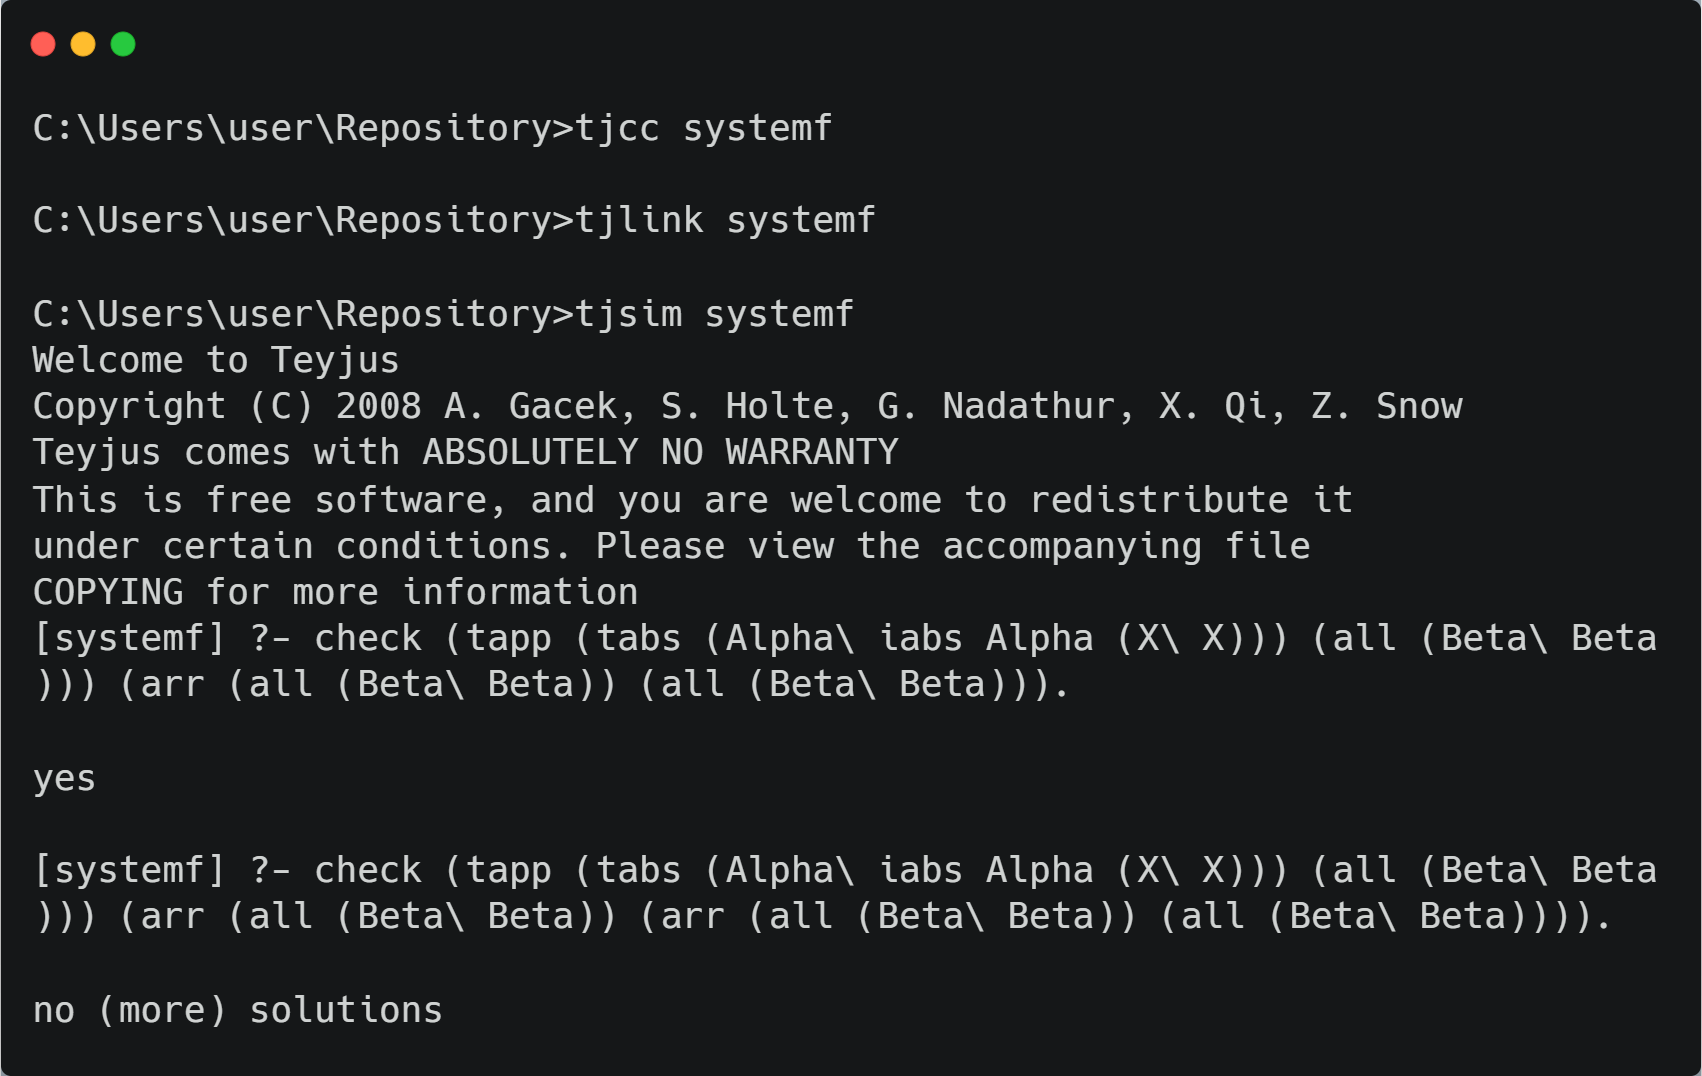
\includegraphics[width=1.0\linewidth]{fin.png}
            \end{center}
        \end{figure}
    \end{frame}

    \begin{frame}
        \frametitle{실행}
        \begin{enumerate}
            \item 먼저, $$\vdash \left( \Lambda \alpha . \lambda x^{\alpha} . x \right) \left( \forall \beta . \beta \right) : \left( \forall \beta . \beta \right) \to \left( \forall \beta . \beta \right)$$인지 질문했는데,
            \item Teyjus는 \texttt{yes}라고 답했네요.
            \item 그 다음, $$\vdash \left( \Lambda \alpha . \lambda x^{\alpha} . x \right) \left( \forall \beta . \beta \right) : \left( \forall \beta . \beta \right) \to \left( \forall \beta . \beta \right) \to \left( \forall \beta . \beta \right)$$인지 질문했는데,
            \item Teyjus는 \texttt{no (more) solutions}라고 답했네요.
            \item 두 경우 모두 예상대로 작동하는 것을 알 수 있습니다.
        \end{enumerate}
    \end{frame}
    
    \begin{frame}[c]
        \frametitle{끝}
        \centering
        지금까지 경청해주셔서 감사합니다!
    \end{frame}
\end{document}
